\appendix

\section{Implementation of NLO QED corrections in APFEL}
\label{sec:appendixAPFEL}

In this appendix we present the details of the implementation of the
combined NLO QCD+QED corrections in the {\tt APFEL} program.
%
As discussed in Ref.~\cite{Bertone:2013vaa}, the implementation of the
LO QED corrections to the DGLAP evolution equations presents many
simplifications, in particular the fact that QED and QCD corrections
do not mix and therefore the DGLAP equations as well as the evolution
equations for $\alpha_s$ and $\alpha$ are decoupled.
%
When going to NLO this property does not hold anymore and QED and QCD
contributions mix both in the DGLAP and in the coupling evolution
equations.
%
On top of this complication, QED corrections induce the presence of
diagrams in which a real photon is present either in the initial or in
the final state and that have to be included in the computation of the
DIS structure functions.

In the following, we first discuss how to generalize the equations for
the running of the QCD and QED couplings, finding that the mixing
QCD+QED terms have a negligible impact.
%
Then we explain how the DGLAP evolution equations can be generalised
to account for the full NLO QCD+QED effects.
%
Finally, we discuss the modifications induced by the NLO QED
corrections in both the neutral-current and the charged-current DIS
structure functions and that lead the appearance of photon-initiated
contributions.

\subsection{Evolution of the couplings}

As mentioned above, the NLO QCD+QED corrections induce the presence of
mixing terms in the evolution equations of $\alpha_s$ and $\alpha$.
%
In practice, the QCD $\beta$-function receives corrections
proportional to $\alpha$ and, vice-versa, the QED $\beta$-function
receives corrections proportional to $\alpha_s$, in such a way that
the coupling evolution equations read:
\begin{equation}\label{CoupledEq}
\begin{array}{rcl}
\displaystyle \mu^2\frac{\partial \alpha_s}{\partial \mu^2} &=& \displaystyle
                                                \beta^{\rm QCD}(\alpha_s,\alpha)\,,\\
\\
\displaystyle \mu^2\frac{\partial \alpha}{\partial \mu^2} &=& \displaystyle \beta^{\rm QED}(\alpha_s,\alpha)\,.
\end{array}
\end{equation}
As a consequence, these evolution equations form a set of coupled
differential equations. Up to three loops ($i.e.$ NLO), the
$\beta$-functions can be expanded as:
\begin{equation}
\beta^{\rm QCD}(\alpha_s,\alpha) = -\alpha_s\left[\beta_0^{(\alpha_s)}\left(\frac{\alpha_s}{4\pi}\right)+\beta_1^{(\alpha_s\alpha)}\left(\frac{\alpha_s}{4\pi}\right) \left(\frac{\alpha}{4\pi}\right)+\beta_1^{(\alpha_s^2)}\left(\frac{\alpha_s}{4\pi}\right)^2+\dots\right]\,,
\end{equation}
and:
\begin{equation}
\beta^{\rm QED}(\alpha_s,\alpha) = -\alpha\left[\beta_0^{(\alpha)}\left(\frac{\alpha}{4\pi}\right)+\beta_1^{(\alpha\alpha_s)}\left(\frac{\alpha}{4\pi}\right) \left(\frac{\alpha_s}{4\pi}\right)+\beta_1^{(\alpha^2)}\left(\frac{\alpha}{4\pi}\right)^2+\dots\right]\,.
\end{equation}
where the mixing terms, $\beta_1^{(\alpha_s\alpha)}$ and
$\beta_1^{(\alpha\alpha_s)}$, and the pure NLO QED term,
$\beta_1^{(\alpha^2)}$, can be found in
Ref.~\cite{Surguladze:1996hx}. Taking into account a factor four due
to the different definitions of the expansion parameters, one finds:
\begin{equation}\label{eq:NewBetaTerms}
\beta_1^{(\alpha_s\alpha)} = -2\sum_{i=1}^{n_f}
e_q^2\,\qquad\beta_1^{(\alpha\alpha_s)} = -\frac{16}{3}N_c\sum_{i=1}^{n_f} e_q^2\,,\qquad \beta_1^{(\alpha^2)} = -4\left(n_l+N_c\sum_{i=1}^{n_f} e_q^2\right)\,,
\end{equation}
where $N_c=3$ is the number of colours, $e_q$ is the electric charge
of the quark flavour $q$, and $n_f$ and $n_l$ are the number of active
quark and lepton flavours, respectively.

Eq.~(\ref{CoupledEq}) can be written in the vectorial form:
\begin{equation}\label{CoupledEqVect}
\mu^2\frac{\partial {\bm \alpha}}{\partial \mu^2} = {\bm \beta}\left({\bm \alpha}(\mu)\right)\,,
\end{equation}
with:
\begin{equation}
  {\bm \alpha} = {\alpha_s \choose \alpha}\qquad\mbox{and}\qquad  {\bm \beta} = {\beta^{\rm QCD} \choose \beta^{\rm QED}}\,.
\end{equation}
Eq.~(\ref{CoupledEqVect}) is an ordinary differential equation that
can be numerically solved using, for example, Runge-Kutta methods.

The first two terms in eq.~(\ref{eq:NewBetaTerms}) are responsible for
the coupling of the evolution of $\alpha_s$ and $\alpha$ and thus they
introduce a complication that affects both the implementation and the
performance of the code. One can then ask what is the effect of their
presence and whether their removal makes a substantial difference. In
Fig.~\ref{fig:CouplingEvol} we show the comparison between the
evolution at NLO of both couplings $\alpha_s$ and $\alpha$ including
and excluding the mixing terms in the respective
$\beta$-functions. The evolution is performed between the $Z$ mass
scale $M_Z$ and 10 TeV with 5 active quark flavours and 3 active
lepton flavours and uses as boundary conditions
$\alpha_s(M_Z) = 0.118$ and $\alpha(M_Z) = 1/128$. The two curves in
Fig.~\ref{fig:CouplingEvol} are normalised to the respective curve
without mixing terms. It is clear that the mixing terms lead to tiny
relative differences that are at most of $\mathcal{O}(10^{-4})$ at 10
TeV for $\alpha_s$ and $\mathcal{O}(10^{-3})$ at the same scale for
$\alpha$. We conclude that the mixing terms in the $\beta$-functions
have a negligible effect on the evolution of the couplings and thus we
exclude them to make the code simpler and improve the performance
without introducing any significant inaccuracy.

%%%%%%%%%%%%%%%%%%%%%%%%%%%%%%%%%%%%%%%%%%%%%%%%%%%%%%%%
\begin{figure}[h]
\includegraphics[width=6cm,angle=270]{figs/couplings.eps} 
\caption{Comparison between the running with the scale
$Q$ of the QCD and QED couplings,
  $\alpha_s$ and $\alpha$, including or not the mixing terms in
  the corresponding $\beta$-functions.
%
  The curves are normalised to the result of the respective coupling
  running without mixing terms.}
\label{fig:CouplingEvol}
\end{figure}
%%%%%%%%%%%%%%%%%%%%%%%%%%%%%%%%%%%%%%%%%%%%%%%%%%%%%%%%

\subsection{PDF evolution with NLO QED corrections}

Next we show how to implement the full NLO QCD+QED corrections to the
DGLAP evolution equations. Here we limit ourselves to consider only
the photon PDF without including leptons.
%
The first step towards an efficient implementation of the solution of
the DGLAP equations in the presence of QED corrections is the adoption
of a suitable PDF basis that diagonalises the splitting function
matrix, decoupling as many equations as possible.
%
Such basis was introduced in the Appendix A of
Ref.~\cite{Bertone:2015lqa} and will be used also here.
%
Excluding the lepton PDFs, this basis contains 14 independent PDF
combinations and reads:
\begin{equation}\label{eq:EvolBasis}
\begin{array}{ll}
\mbox{\texttt{ 1} : }g & \\
\mbox{\texttt{ 2} : }\gamma & \\
\mbox{\texttt{ 3} : }\displaystyle \Sigma = \Sigma_u + \Sigma_d & \quad
\mbox{\texttt{9} : }\displaystyle V =V_u +  V_d\\
\mbox{\texttt{ 4} : } \displaystyle \Delta_\Sigma = \Sigma_u - \Sigma_d& \quad\displaystyle 
\mbox{\texttt{10} : } \Delta_V = V_u - V_d\\
\mbox{\texttt{ 5} : }T_1^u = u^+ - c^+ &\quad \mbox{\texttt{11} : }V_1^u = u^- - c^- \\
\mbox{\texttt{ 6} : }T_2^u = u^+ + c^+ - 2t^+ &\quad \mbox{\texttt{12} : }V_2^u = u^- + c^- - 2t^-\\
\mbox{\texttt{ 7} : }T_1^d = d^+ - s^+ &\quad \mbox{\texttt{13} : }V_1^d = d^- - s^- \\
\mbox{\texttt{ 8} : }T_2^d = d^+ + s^+ - 2b^+ &\quad \mbox{\texttt{14}
                                               : }V_2^d = d^- + s^- -
                                               2b^-\\
\end{array}
\end{equation}
where we have defined $q^\pm = q\pm\overline{q}$ with
$q = u,d,s,c,b,t$. In addition, we have defined:
\begin{equation}
\begin{array}{ll}
\Sigma_u = u^++c^++t^+, &\quad V_u = u^-+c^-+t^-,\\
\\
\Sigma_d = d^++s^++b^+,&\quad V_d = d^-+s^-+b^-\,.
\end{array}
\end{equation}

The second step is the construction the splitting function matrix that
determines the evolution of each of the combinations listed in
Eq.~(\ref{eq:EvolBasis}).
%
To this end, we split the splitting function matrix $P$ into a pure
QCD term $\widetilde{P}$, which only depends on $\alpha_s$, and a
mixed QCD+QED correction term $\overline{P}$, which instead contains
contributions proportional to at least one power of the QED coupling
$\alpha$.
%
In practice, this means that
\begin{equation}
P = \widetilde{P} + \overline{P}\,,
\end{equation}
where the pure QCD term reads:
\begin{equation}\label{eq:PureQCDSplittings}
\widetilde{P} = \alpha_s \mathcal{P}^{(1,0)} + \alpha_s^2 \mathcal{P}^{(2,0)}+\dots\, ,
\end{equation}
while the term containing the QED coupling is given by:
\begin{equation}\label{eq:QCD+QEDSplittings}
\overline{P} = \alpha \mathcal{P}^{(0,1)} + \alpha_s\alpha \mathcal{P}^{(1,1)}+\alpha^2 \mathcal{P}^{(0,2)} + \dots \, .
\end{equation}
Note that in the r.h.s. of Eqs.~(\ref{eq:PureQCDSplittings})
and~(\ref{eq:QCD+QEDSplittings}) we are following the convention of
Refs.~\cite{deFlorian:2015ujt,deFlorian:2016gvk} to indicate the power
of $\alpha_s$ and $\alpha$ that each splitting function multiplies.

The structure of the pure QCD splitting function matrix
$\widetilde{P}$ as well as the first term in $\overline{P}$, which
represents the pure LO QED correction, were already discussed in
Ref.~\cite{Bertone:2015lqa}.
%
It is now necessary to analyse the structure of the two additional
terms, namely $\mathcal{P}^{(1,1)}$ and $\mathcal{P}^{(0,2)}$.
%
Let us start with the $\mathcal{O}(\alpha_s\alpha)$ term.
%
At this perturbative order, the resulting evolution equations read:
\begin{equation}
\begin{array}{rcl}
\displaystyle\left.\mu^2\frac{\partial}{\partial \mu^2}
\begin{pmatrix}
g\\
\gamma\\
\Sigma\\
\Delta_\Sigma
\end{pmatrix}
\right|_{\mathcal{O}(\alpha_s \alpha)} &=& \displaystyle \begin{pmatrix}
e_\Sigma^2 \mathcal{P}^{(1,1)}_{gg}      & e_\Sigma^2 \mathcal{P}^{(1,1)}_{g\gamma} & \eta^+\mathcal{P}^{(1,1)}_{gq} & \eta^-\mathcal{P}^{(1,1)}_{gq} \\
e_\Sigma^2 \mathcal{P}^{(1,1)}_{\gamma g} & e_\Sigma^2 \mathcal{P}^{(1,1)}_{\gamma\gamma} & \eta^+\mathcal{P}^{(1,1)}_{\gamma q} &\eta^-\mathcal{P}^{(1,1)}_{\gamma q} \\
2 e_\Sigma^2 \mathcal{P}^{(1,1)}_{qg}    & 2 e_\Sigma^2 \mathcal{P}^{(1,1)}_{q\gamma} & \eta^+\mathcal{P}^{+(1,1)}  & \eta^-\mathcal{P}^{+(1,1)}\\
2 \delta_e^2 \mathcal{P}^{(1,1)}_{qg} & 2 \delta_e^2 \mathcal{P}^{(1,1)}_{q\gamma} &\eta^-\mathcal{P}^{+(1,1)} &\eta^+\mathcal{P}^{+(1,1)}
\end{pmatrix}\otimes
\begin{pmatrix}
g\\
\gamma\\
\Sigma\\
\Delta_\Sigma
\end{pmatrix}
\end{array}\,,
\end{equation}

\begin{equation}
\displaystyle\left.\mu^2\frac{\partial}{\partial \mu^2}
\begin{pmatrix}
V\\
\Delta_V
\end{pmatrix} \right|_{\mathcal{O}(\alpha_s \alpha)}= 
\begin{pmatrix}
\eta^+\mathcal{P}^{-(1,1)} & \eta^-\mathcal{P}^{-(1,1)} \\
\eta^-\mathcal{P}^{-(1,1)} & \eta^+\mathcal{P}^{-(1,1)} 
\end{pmatrix}\otimes
\begin{pmatrix}
V\\
\Delta_V
\end{pmatrix}\,,
\end{equation}

\begin{equation}
\begin{array}{ll}
\begin{array}{rcl}
\displaystyle \left.\mu^2\frac{\partial T^u_{1,2}}{\partial \mu^2}\right|_{\mathcal{O}(\alpha_s \alpha)} &=&
\displaystyle e_u^2\mathcal{P}^{+(1,1)}\otimes T^u_{1,2}
\end{array}\,, &
\begin{array}{rcl}
\displaystyle \left.\mu^2\frac{\partial T^d_{1,2}}{\partial \mu^2}\right|_{\mathcal{O}(\alpha_s \alpha)} &=&
\displaystyle e_d^2\mathcal{P}^{+(1,1)} \otimes T^d_{1,2}
\end{array}\,,
\\
\\
\begin{array}{rcl}
\displaystyle \left.\mu^2\frac{\partial V^u_{1,2}}{\partial \mu^2}\right|_{\mathcal{O}(\alpha_s \alpha)} &=&
\displaystyle e_u^2\mathcal{P}^{-(1,1)} \otimes V^u_{1,2}
\end{array}\,, &
\begin{array}{rcl}
\displaystyle \left.\mu^2\frac{\partial V^d_{1,2}}{\partial \mu^2}\right|_{\mathcal{O}(\alpha_s \alpha)} &=&
\displaystyle e_d^2\mathcal{P}^{-(1,1)}\otimes V^d_{1,2}
\end{array}\,.
\end{array}
\end{equation}
where $\otimes$ indicates the Mellin convolution and where we have
defined:
\begin{equation}
\begin{array}{rcl}
e_{\Sigma}^{2}& \equiv &\displaystyle
N_c(n_ue_{u}^{2}+n_de_{d}^{2})\,,\\
\\
\delta_e^2 & \equiv &\displaystyle N_c(n_u e_u^2 -n_d e_d^2)\,,\\
\\
\eta^{\pm} & \equiv & \displaystyle \frac{1}{2}\left(e_{u}^{2}\pm
  e_{d}^{2}\right)\,,\\
\end{array}
\end{equation}
with $e_u$ and $e_d$ the electric charges of the up- and down-type
quarks, and $n_u$ and $n_d$ the number of up- and down-type active
quark flavours (such that $n_u+n_d=n_f$).
%
%Once expressed this basis, it is possible to include the
%$\mathcal{O}(\alpha_s\alpha)$ corrections in the solution of the DGLAP
%QCD+QED equations in APFEL as done in Ref.~\cite{Bertone:2015lqa}.

Now we turn to consider the $\mathcal{O}(\alpha^2)$ corrections.
%
The expressions of the splitting functions at this order have been
presented in Ref.~\cite{deFlorian:2016gvk}.
%
There are two relevant new features that distinguish these corrections
from the $\mathcal{O}(\alpha)$ and the $\mathcal{O}(\alpha_s\alpha)$
ones.
%
The first one is that, contrary to the other cases in which the
electric charges appears to the second power at most, here they appear
up to the fourth power.
%
As a consequence, we need to introduce the new couplings:
\begin{equation}
\begin{array}{l}
e_{\Sigma}^4 = N_c(n_{u} e_u^4 + n_{d} e_d^4)\,,\\
\\
\delta_e^4 = N_c(n_{u} e_u^4 - n_{d} e_d^4)\,.
\end{array}
\end{equation}
The second feature is that the dependence on the electric charges of
some of the $\mathcal{O}(\alpha^2)$ splitting functions is not
factorisable as it was the case for all the $\mathcal{O}(\alpha)$ and
$\mathcal{O}(\alpha_s\alpha)$ ones, and therefore we need to
distinguish between up- and down-type splitting functions.
%
Taking into account these features, it is possible to show that the
$\mathcal{O}(\alpha^2)$ contributions to the DGLAP equations take the
following form:
\begin{equation}
%\begin{array}{rcl}
\begin{array}{c}
\displaystyle\left.\mu^2\frac{\partial}{\partial \mu^2}
\begin{pmatrix}
g\\
\gamma\\
\Sigma\\
\Delta_\Sigma
\end{pmatrix}
  \right|_{\mathcal{O}(\alpha^2)} =\\
\\
 \displaystyle \frac12\begin{pmatrix}
    0 & 0 & 0 & 0 \\
    0 & 2e_\Sigma^4 \mathcal{P}_{\gamma\gamma}^{(0,2)} & e_u^4 \mathcal{P}_{\gamma
      u}^{(0,2)} + e_d^4 \mathcal{P}_{\gamma d} & e_u^4 \mathcal{P}_{\gamma u}^{(0,2)} - e_d^4 \mathcal{P}_{\gamma d}^{(0,2)}\\
    0 & 4 e_\Sigma^4 \mathcal{P}^{(0,2)}_{q\gamma} &
    e_u^4\mathcal{P}_{uu}^{+(0,2)}
    +e_d^4\mathcal{P}_{dd}^{+(0,2)}+2\eta^+e_\Sigma^2\mathcal{P}^{S(0,2)}_{qq} & e_u^4\mathcal{P}_{uu}^{+(0,2)}-e_d^4\mathcal{P}_{dd}^{+(0,2)} + 2\eta^-e_\Sigma^2\mathcal{P}^{S(0,2)}_{qq}\\
    0 & 4 \delta_e^4 \mathcal{P}^{(0,2)}_{q\gamma} & e_u^4\mathcal{P}_{uu}^{+(0,2)}
    -e_d^4\mathcal{P}_{dd}^{+(0,2)}+2\eta^-\delta_e^2
    \mathcal{P}^{S(0,2)}_{qq} & e_u^4\mathcal{P}_{uu}^{+(0,2)}+e_d^4\mathcal{P}_{dd}^{+(0,2)} + 2\eta^+\delta_e^2 \mathcal{P}^{S(0,2)}_{qq}
\end{pmatrix}\otimes
\begin{pmatrix}
g\\
\gamma\\
\Sigma\\
\Delta_\Sigma
\end{pmatrix}\,,
\end{array}
\end{equation}

\begin{equation}
\displaystyle\left.\mu^2\frac{\partial}{\partial \mu^2}
\begin{pmatrix}
V\\
\Delta_V
\end{pmatrix} \right|_{\mathcal{O}(\alpha^2)}= \frac12
\begin{pmatrix}
e_u^4\mathcal{P}_{uu}^{-(0,2)}+e_d^4\mathcal{P}_{dd}^{-(0,2)} & e_u^4\mathcal{P}_{uu}^{-(0,2)}-e_d^4\mathcal{P}_{dd}^{-(0,2)} \\
e_u^4\mathcal{P}_{uu}^{-(0,2)}-e_d^4\mathcal{P}_{dd}^{-(0,2)} & e_u^4\mathcal{P}_{uu}^{-(0,2)}+e_d^4\mathcal{P}_{dd}^{-(0,2)} 
\end{pmatrix}\otimes
\begin{pmatrix}
V\\
\Delta_V
\end{pmatrix}\,,
\end{equation}

\begin{equation}
\begin{array}{ll}
\begin{array}{rcl}
\displaystyle \left.\mu^2\frac{\partial T^u_{1,2}}{\partial \mu^2}\right|_{\mathcal{O}(\alpha^2)} &=&
\displaystyle e_u^4\mathcal{P}_{uu}^{+(0,2)}\otimes T^u_{1,2}
\end{array}\,, &
\begin{array}{rcl}
\displaystyle \left.\mu^2\frac{\partial T^d_{1,2}}{\partial \mu^2}\right|_{\mathcal{O}(\alpha^2)} &=&
\displaystyle e_d^4\mathcal{P}_{dd}^{+(0,2)} \otimes T^d_{1,2}
\end{array}\,,
\\
\\
\begin{array}{rcl}
\displaystyle \left.\mu^2\frac{\partial V^u_{1,2}}{\partial \mu^2}\right|_{\mathcal{O}(\alpha^2)} &=&
\displaystyle e_u^4\mathcal{P}_{uu}^{-(0,2)} \otimes V^u_{1,2}
\end{array}\,, &
\begin{array}{rcl}
\displaystyle \left.\mu^2\frac{\partial V^d_{1,2}}{\partial \mu^2}\right|_{\mathcal{O}(\alpha^2)} &=&
\displaystyle e_d^4\mathcal{P}_{dd}^{-(0,2)}\otimes V^d_{1,2}
\end{array}\,.
\end{array}
\end{equation}
It should be noted that, as compared to the expressions for
$\mathcal{P}^{(0,2)}$ presented in Ref.~\cite{deFlorian:2016gvk}, we
have factored out the electric charges in such a way that the
expressions of the splitting functions are either independent from the
electric charges or depend on them only through the ratio
$e_\Sigma^2/e_q^2$.
%
%As before, once the $\mathcal{O}(\alpha^2)$ corrections to the QCD+QED
%combined evolution equations are expressed in this form, it is
%possible to include them in {\tt APFEL} and to solve them using the
%same numerical techniques as for the other cases.

As an illustration, we have quantified the effects of the
$\mathcal{O}(\alpha_s\alpha)$ and $\mathcal{O}(\alpha^2)$ corrections
to the DGLAP evolution equations on the $\gamma\gamma$ luminosity at
$\sqrt{s} = 13$ TeV, defined as:
\begin{equation}\label{eq:GammaGammaLumi}
\mathcal{L}_{\gamma\gamma}(M_X) = \frac1{s}\int_{M_X^2/s}^1
\frac{dx}{x} \gamma(x,M_X) \gamma\left(\frac{M_X^2}{xs},M_X\right)\,,
\end{equation}
as a function of the final state invariant mass $M_X$.
%
Fig.~\ref{fig:GammaGammaLumi} illustrates the behaviour of
$\mathcal{L}_{\gamma\gamma}$ computed using the photon PDF from the
NNPDF30QED NLO set as an input at $Q_0 = 1$ GeV and evolved to $Q=M_X$
including, on top of the pure QCD NLO evolution, the following
corrections:
\begin{itemize}
\item the $\mathcal{O}(\alpha)$ corrections only,
\item same as above, adding also the mixing
  $\mathcal{O}(\alpha_s\alpha)$ corrections, and
\item the complete NLO QCD+QED corrections accounting for the
  $\mathcal{O}(\alpha+\alpha_s\alpha+\alpha^2)$ effects.
\end{itemize}
The results are shown normalised to the predictions obtained with LO
QED corrections only.
%
It is clear that the $\mathcal{O}(\alpha_s\alpha)$ and
$\mathcal{O}(\alpha^2)$ corrections have a small but non-negligible
impact on the $\gamma\gamma$-luminosity. In particular, these
corrections suppress $\mathcal{L}_{\gamma\gamma}$ by almost 5\% at
relatively small values of $M_X$, while the suppression gradually
shrinks to 1-2\% as $M_X$ increases. As expected, most of this effect
comes from the $\mathcal{O}(\alpha_s\alpha)$ corrections, while the
impact of the $\mathcal{O}(\alpha^2)$ ones is substantially smaller.

%%%%%%%%%%%%%%%%%%%%%%%%%%%%%%%%%%%%%%%%%%%%%%%%%%%%%%%%
\begin{figure}[t]
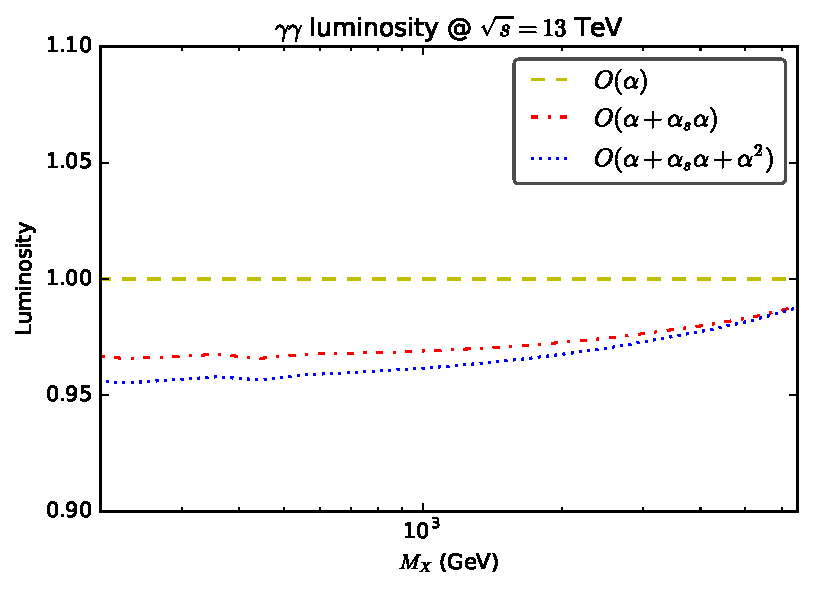
\includegraphics[width=8cm]{figs/lumi_13tev.pdf} 
\caption{The photon-photon PDF luminosity $\mathcal{L}_{\gamma\gamma}$ at $\sqrt{s} = 13$ TeV as a
  function of the final state invariant mass $M_X$.
  %
  We compare the results of the photon evolved
  with only the $\mathcal{O}(\alpha)$ corrections
  with the corresponding results taking into account the 
  $\mathcal{O}(\alpha+\alpha_s\alpha)$ corrections
  and the complete
  $\mathcal{O}(\alpha+\alpha_s\alpha+\alpha^2)$ effects,
  normalised to the $\mathcal{O}(\alpha)$ result.
  %
  The calculation has been performed using NNPDF3.0QED NLO.  }
\label{fig:GammaGammaLumi}
\end{figure}
%%%%%%%%%%%%%%%%%%%%%%%%%%%%%%%%%%%%%%%%%%%%%%%%%%%%%%%%

\subsection{DIS structure functions}

When considering NLO QCD+QED corrections to the DIS structure
functions, it becomes necessary to include into the hard cross
sections all the $\mathcal{O}(\alpha)$ diagrams where one photon is
either in the initial state or emitted from an incoming quark (or
possibly an incoming lepton).
%
Such diagrams, being of purely QED origin, have associated coefficient
functions that can be easily derived from the QCD expressions by
properly adjusting the colour factors.
%
This correspondence holds irrespective of whether mass effects are
included.

The main complication of the inclusion of these corrections arises
from their flavour structure. In fact, due to the fact that the
coupling of the photon is proportional to the squared charge of the
parton to which it couples (a quark or a lepton), in the case of
quarks the isospin symmetry is broken.
%
In the following, we will address separately the neutral-current (NC)
case, where lepton and proton exchange a neutral boson $\gamma^*/Z$,
and the charged-current (CC) case, where instead lepton and proton
exchange a charged $W$ boson.

First of all, let us concentrate on the $\mathcal{O}(\alpha)$
contributions to a generic NC structure function $F$.
%
Due to the fact that to this order there is no mixing between QCD and
QED, such corrections can easily be derived from the
$\mathcal{O}(\alpha_s)$ coefficient functions just by adjusting the
colour factors by setting $C_F=T_R=1$ and $C_A=0$.
%
Referring, $e.g.$, to the expressions reported in
Ref.~\cite{Ellis:1991qj}, one has that:
\begin{equation}\label{eq:alphaCFs}
\begin{array}{rcl}
\displaystyle C_{i;q}^{(\alpha)} &=& \displaystyle \frac{C_{i;q}^{(\alpha_s)}}{C_F}\\
\\
\displaystyle C_{i;\gamma}^{(\alpha)} &=& \displaystyle \frac{C_{i;g}^{(\alpha_s)}}{T_R}
\end{array}\qquad i = 2,L,3\,.
\end{equation}
In addition, in order to construct the corresponding structure
functions, considering that the coupling between a photon and a quark
of flavour $q$ is proportional to $e_q^2$, one also needs to adjust
the electroweak couplings as follows:
 \begin{equation}
\begin{array}{rcl}
\widetilde{B}_q &=& B_qe_q^2\quad\mbox{for}\quad F_2,F_L\,, \\
\\
\widetilde{D}_q &=& D_qe_q^2\quad\mbox{for}\quad F_3\,, \\
\end{array}
\end{equation}
where $B_q$ and $D_q$ are defined, $e.g.$, in
Ref.~\cite{Adloff:2003uh}.
%
Following this prescription, it is possible to write the
$\mathcal{O}(\alpha)$ contributions to the NC structure functions as:
\begin{equation}
\begin{array}{rcl}
F_{2,L}^{{\rm NC},(\alpha)} &=& \displaystyle x \sum_{q} \widetilde{B}_q\left[C_{2,L;q}^{(\alpha)}\otimes
(q+\overline{q}) + C_{2,L;\gamma}^{(\alpha)} \otimes \gamma
                         \right]\,,\\
\\
F_3^{{\rm NC},(\alpha)} &=& \displaystyle x \sum_{q} \widetilde{D}_q\left[C_{3;q}^{(\alpha)}\otimes
(q-\overline{q}) + C_{3;\gamma}^{(\alpha)} \otimes \gamma
                         \right]\,.
\end{array}
\end{equation}
We emphasise that this structure holds for both massless and massive
structure functions. This aspect is relevant to the construction of
the FONLL general-mass structure functions.

We now move to the CC case, where the procedure to obtain the
expressions of the $\mathcal{O}(\alpha)$ coefficient functions is
exactly the same as in the NC case (see
Eq.~(\ref{eq:alphaCFs})). However, this case is more complicated
because the flavour structure of CC structure functions is more
complex.
%
Taking into account the presence of a factor $e_q^2$ every time that a
quark of flavour $q$ couples to a photon, the $\mathcal{O}(\alpha)$
corrections to the CC structure functions $F_2$ and $F_L$ for the
productions of a neutrino or an anti-neutrino take the form:
\begin{equation}\label{compactNu}
\begin{array}{rcl}
F_{2,L}^{{\rm CC},\nu,(\alpha)} &=& \displaystyle
                              \sum_{U=u,c,t}\sum_{D=d,s,b}|V_{UD}|^2\left[C_{2,L;q}^{(\alpha)}\otimes\left(e_D^2D +e_U^2\overline{U}\right) +2 C_{2,L;\gamma}^{(\alpha)}\otimes\gamma\right]\,,\\
\\
F_{2,L}^{{\rm CC},\overline{\nu},(\alpha)} &=& \displaystyle
\sum_{U=u,c,t}\sum_{D=d,s,b}|V_{UD}|^2\left[C_{2,L;q}^{(\alpha)}\otimes\left(e_D^2\overline{D}
    +e_U^2U\right) +2 C_{2,L;\gamma}^{(\alpha)}\otimes\gamma\right]\,,
\end{array}
\end{equation}
where $V_{UD}$ are the elements of the CKM matrix.
%
The flavour structure of $F_3$ is instead slightly different:
\begin{equation}\label{compactNuF3}
\begin{array}{rcl}
F_3^{{\rm CC},\nu,(\alpha)} &=& \displaystyle
                              \sum_{U=u,c,t}\sum_{D=d,s,b}|V_{UD}|^2\left[C_{3;q}^{(\alpha)}\otimes\left(e_D^2D -e_U^2\overline{U}\right) +2 C_{3;\gamma}^{(\alpha)}\otimes\gamma\right]\,,\\
\\
F_3^{{\rm CC},\overline{\nu},(\alpha)} &=& \displaystyle
\sum_{U=u,c,t}\sum_{D=d,s,b}|V_{UD}|^2\left[C_{3;q}^{(\alpha)}\otimes\left(-e_D^2\overline{D}
    +e_U^2U\right) +2 C_{3;\gamma}^{(\alpha)}\otimes\gamma\right]\,.
\end{array}
\end{equation}
In order to simplify the implementation, it is advantageous to assume
that, in these particular corrections, the CKM matrix is a 3 times 3
unitary matrix. Note however that the exact CKM matrix is still used
in the QCD part of the structure functions.
%
This approximation introduces an inaccuracy of the order of the QED
coupling $\alpha$ times the value of the off-diagonal elements of the
CKM matrix and therefore it is numerically negligible.

As an illustration of the impact of the $\mathcal{O}(\alpha)$
correction on the DIS structure functions, Fig.~\ref{fig:StructFuncs}
shows the effect of introducing these contributions on top of the pure
QCD computation at NLO. The plots are produced by evolving the
NNPDF3.0QED NLO set from $Q_0=1$ GeV to $Q=100$ GeV including the full
NLO QCD+QED corrections discussed in the previous section and using
the resulting evolved PDFs to compute the NC (left panel) and the CC
(right panel) DIS structure functions in the FONLL-B scheme, including
the $\mathcal{O}(\alpha)$ corrections to the coefficient functions
discussed above.
%
The predictions are shown normalised to the pure QCD computation where
the QED corrections are absent both in the evolution and in the
computation of the structure functions.

%%%%%%%%%%%%%%%%%%%%%%%%%%%%%%%%%%%%%%%%%%%%%%%%%%%%%%%%
\begin{figure}[t]
\includegraphics[width=6cm,angle=270]{figs/NLOQEDCorrections_NC.eps}
\includegraphics[width=6cm,angle=270]{figs/NLOQEDCorrections_CC.eps}
\caption{The effects of the NLO QED corrections on the neutral-current
(left) and charged-current (right) DIS structure functions
$F_2, F_3$ and $F_L$, normalised to the pure QCD results.
%
The calculation has been performed in the FONLL-B general-mass scheme using the NNPDF3.0QED NLO
set.
%
Note that QED effects enter both via DGLAP evolution and the
$\mathcal{O}(\alpha)$ DIS coefficient functions.}
\label{fig:StructFuncs}
\end{figure}
%%%%%%%%%%%%%%%%%%%%%%%%%%%%%%%%%%%%%%%%%%%%%%%%%%%%%%%%

It is clear that the impact of the full NLO QCD+QED corrections is
pretty small especially in the low-$x$ region where it is well below
1\%. In the large-$x$ region, instead, the presence of a
photon-initiated contribution has a more significant effect because of
the suppression of the QCD distributions (quarks and gluon) relative
to the photon PDF and the impact of the QED corrections reaches the
2\% level.  It should be stressed that the behaviour around
$x=10^{-2}$ of the CC $F_3$ (green curve in the right panel) is driven
by a change of sign of the predictions so that the ratio diverges.
